\section*{Aufgabe 1}
\subsection*{Mittelwerte}

Die Mittelwerte der drei Populationen
\begin{equation}
  \mu_\text{P1} = \begin{pmatrix} 6.01 \\ 3.01 \end{pmatrix} \text{ , } \mu_{P-0-10000} = \begin{pmatrix} 0.03 \\ 3.03 \end{pmatrix} \text{ und } \mu_{P-0-1000} = \begin{pmatrix} 0.01 \\ 3.01 \end{pmatrix}
\end{equation}
\subsection*{Kovarianzmatrizen}
Die Summierten Kovarianzmatrizen sind
\begin{equation}
  S^{P0} = \begin{pmatrix} 121388.56 & 81082.17 \\ 81082.17 & 66628.71 \end{pmatrix} \text{ und } S^{P1} = \begin{pmatrix} 123917.64 & 8719.56 \\ 8719.56 & 43976.48 \end{pmatrix}
\end{equation}
Die Summierte Kovarianzmatrix hat die From
\begin{equation}
  S^{P01,P00} = \begin{pmatrix} 245306.20 & 898011.72 \\ 89801.72 & 110605.19 \end{pmatrix}
\end{equation}
\subsection*{Fisher-Diskriiminante}
Die Fisherdiskrimante $\lambda$ beträgt
\begin{equation}
  \lambda = \begin{pmatrix} -0.77 \\ 0.63 \end{pmatrix}
\end{equation}
Die Gradengleichung ergibt sich somit zu
\begin{equation}
  f(x) = -0.82 \cdot x \text{    bzw    } x_i = \lambda^T \vec{x}_i
\end{equation}
\subsection*{Population}
\begin{figure}[H]
  \centering
  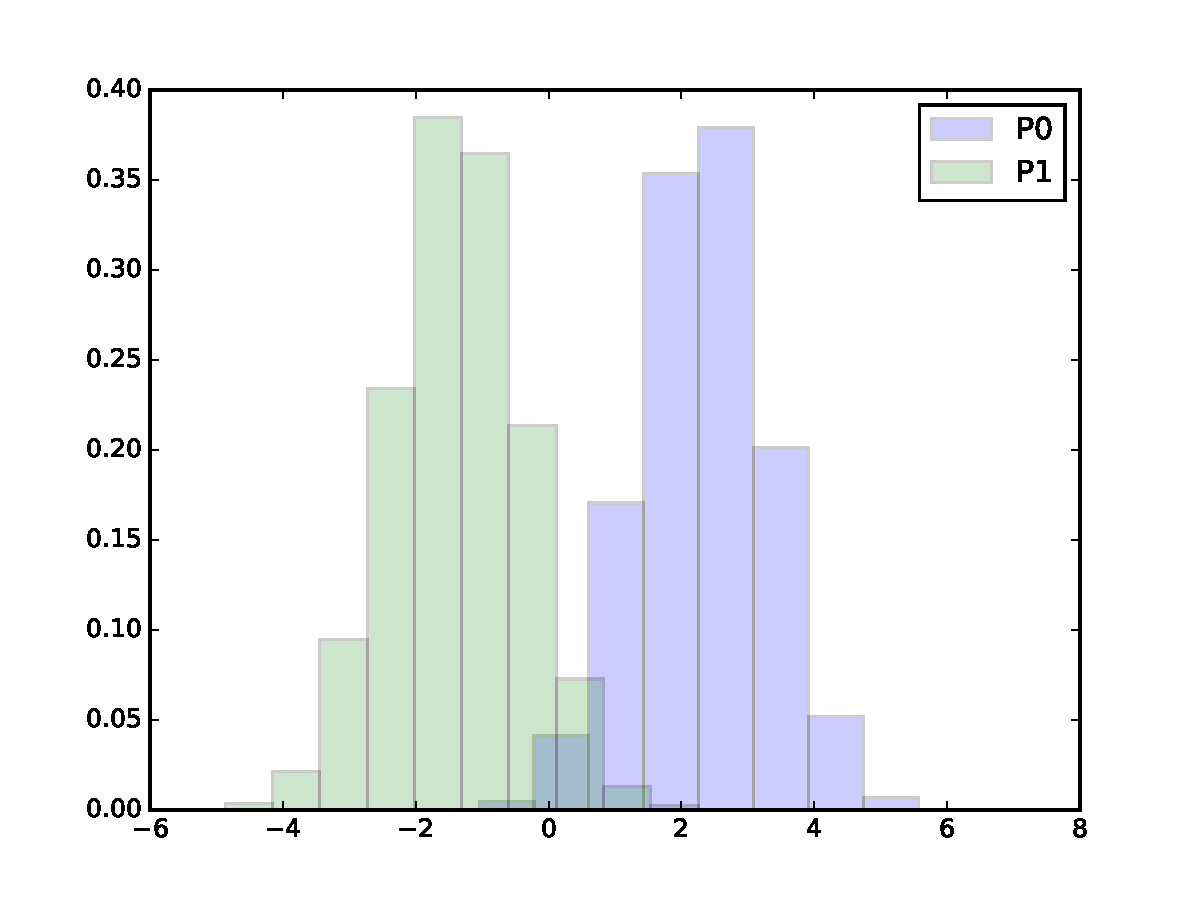
\includegraphics[height=7cm]{./Figures/firstHist.pdf}
  \caption{Abbildung der Populstionen auf die Grade}
\end{figure}
\subsection*{Reinheit}
\begin{figure}[H]
  \centering
  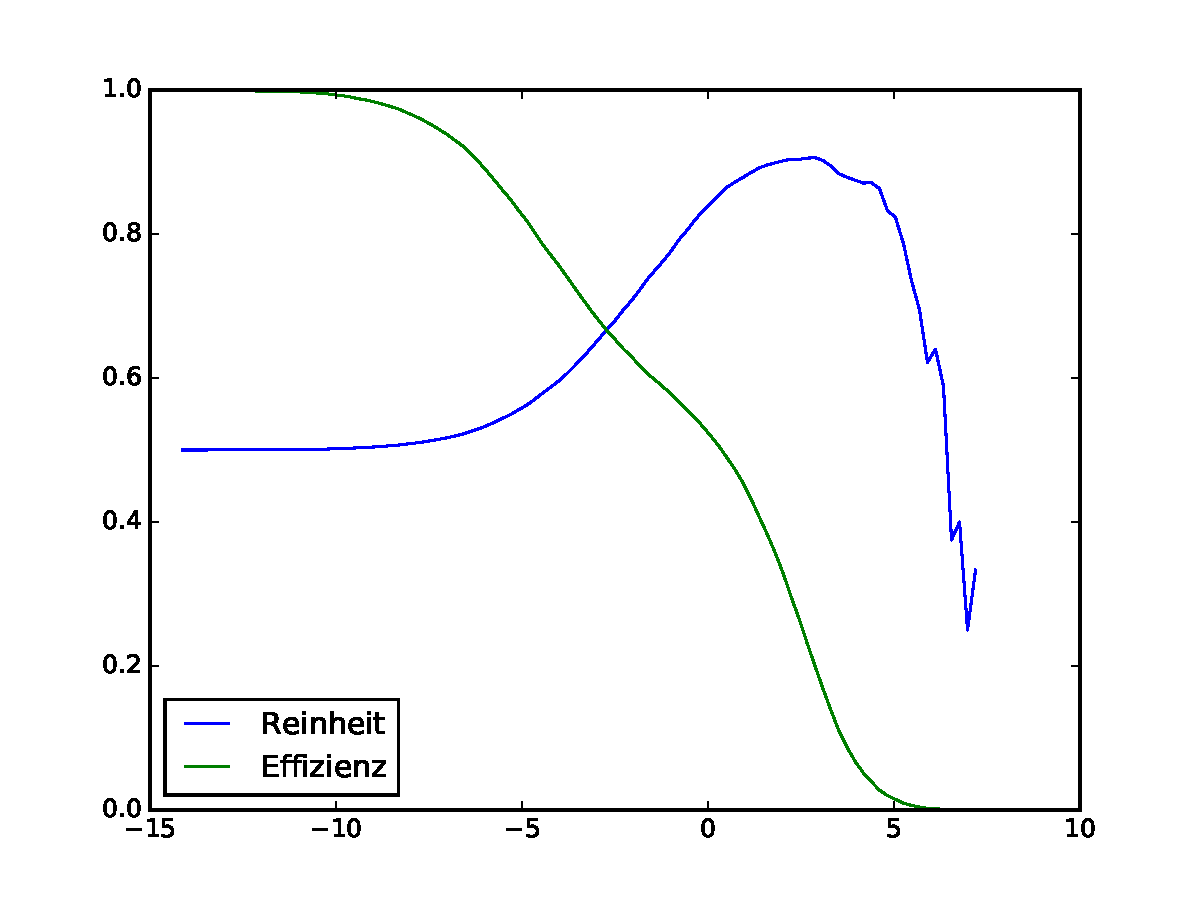
\includegraphics[height=7cm]{./Figures/reinheit1.pdf}
  \caption{Reinheit in Abhängigkeit des Schnittes}
\end{figure}
\subsection*{Signal zu Untergrundverhältnis}
\begin{figure}[H]
  \centering
  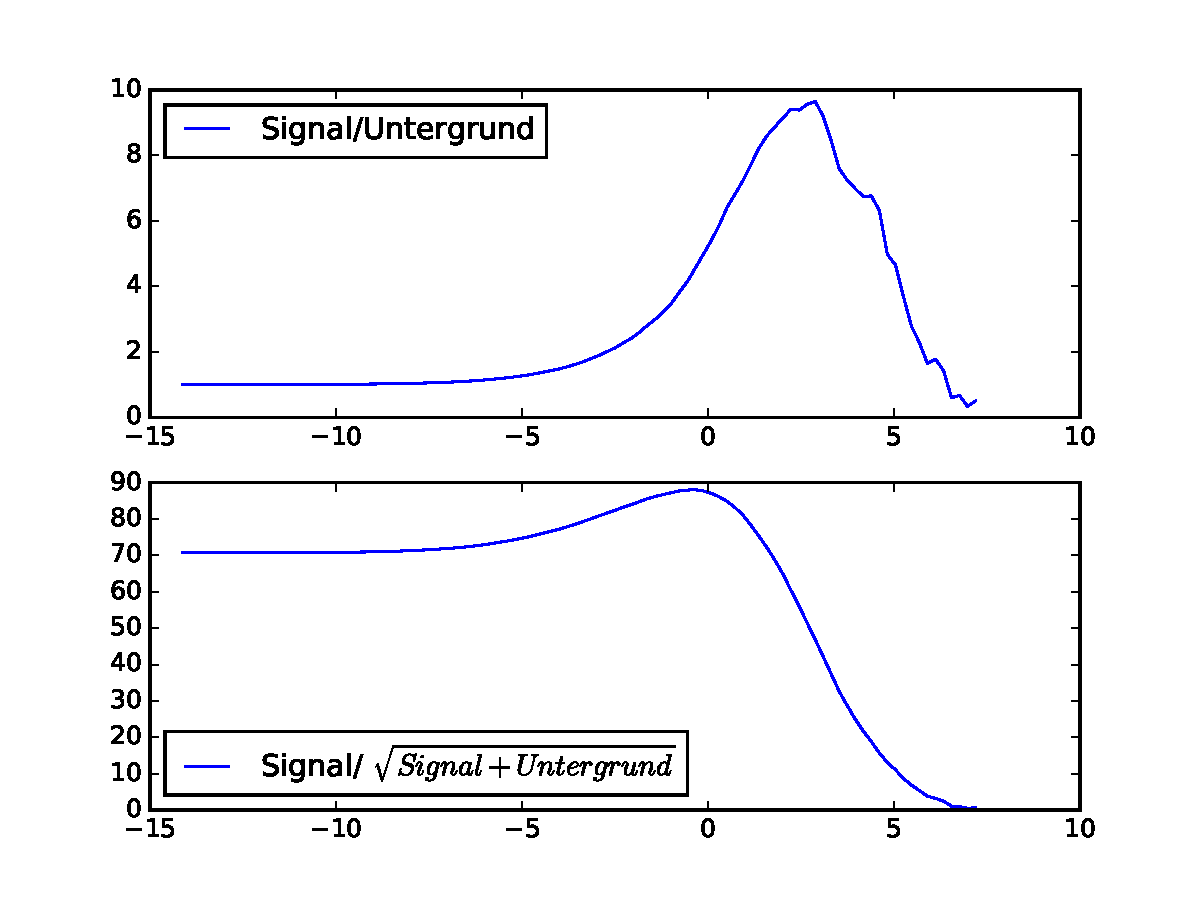
\includegraphics[height=7cm]{./Figures/SigZuUnt1.pdf}
  \caption{Signal zu Untergrundverhältnis sowie Signifikanz}
\end{figure}

\subsection*{Für die andere Population}

\begin{figure}[H]
  \centering
  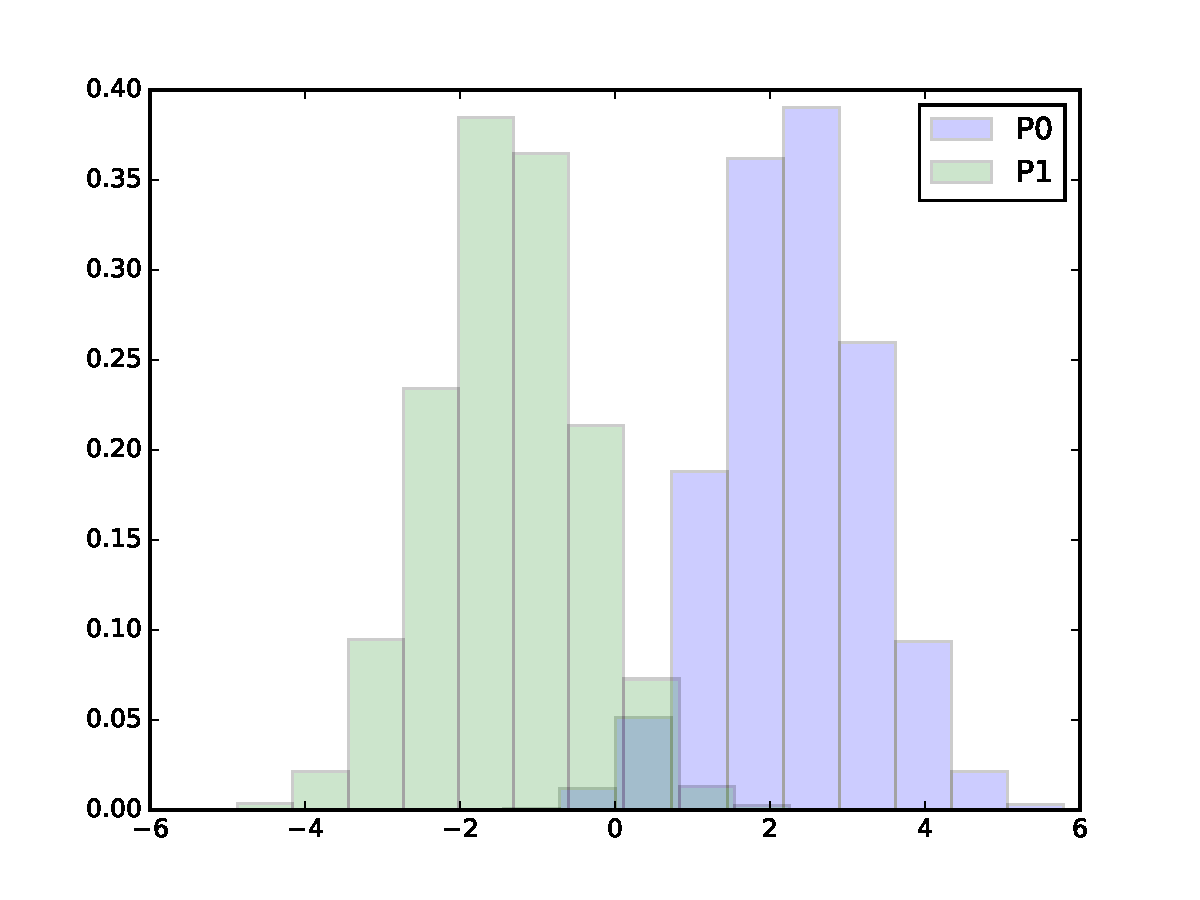
\includegraphics[height=7cm]{./Figures/secondHist.pdf}
  \caption{Abbildung der Populstionen auf die Grade}
\end{figure}

\begin{figure}[H]
  \centering
  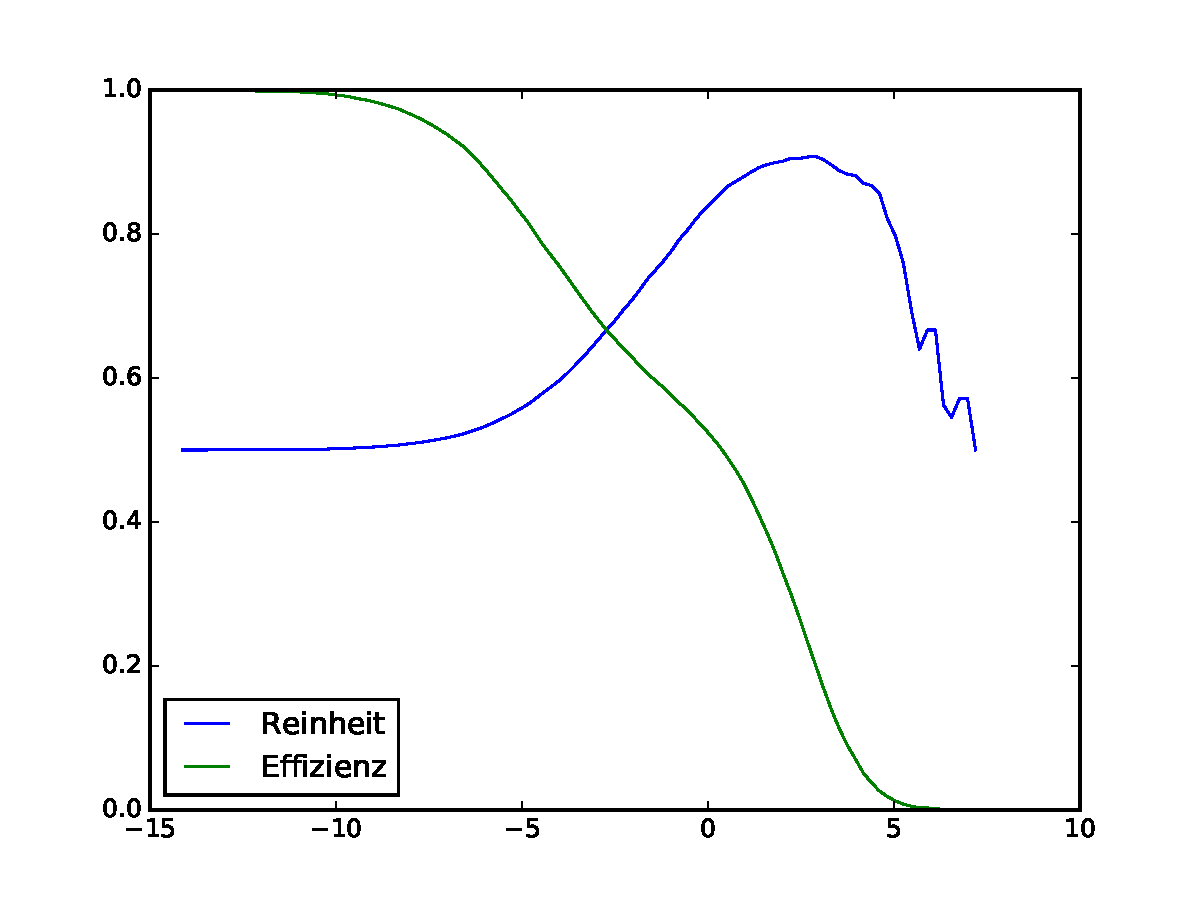
\includegraphics[height=7cm]{./Figures/reinheit2.pdf}
  \caption{Reinheit in Abhängigkeit des Schnittes}
\end{figure}

\begin{figure}[H]
  \centering
  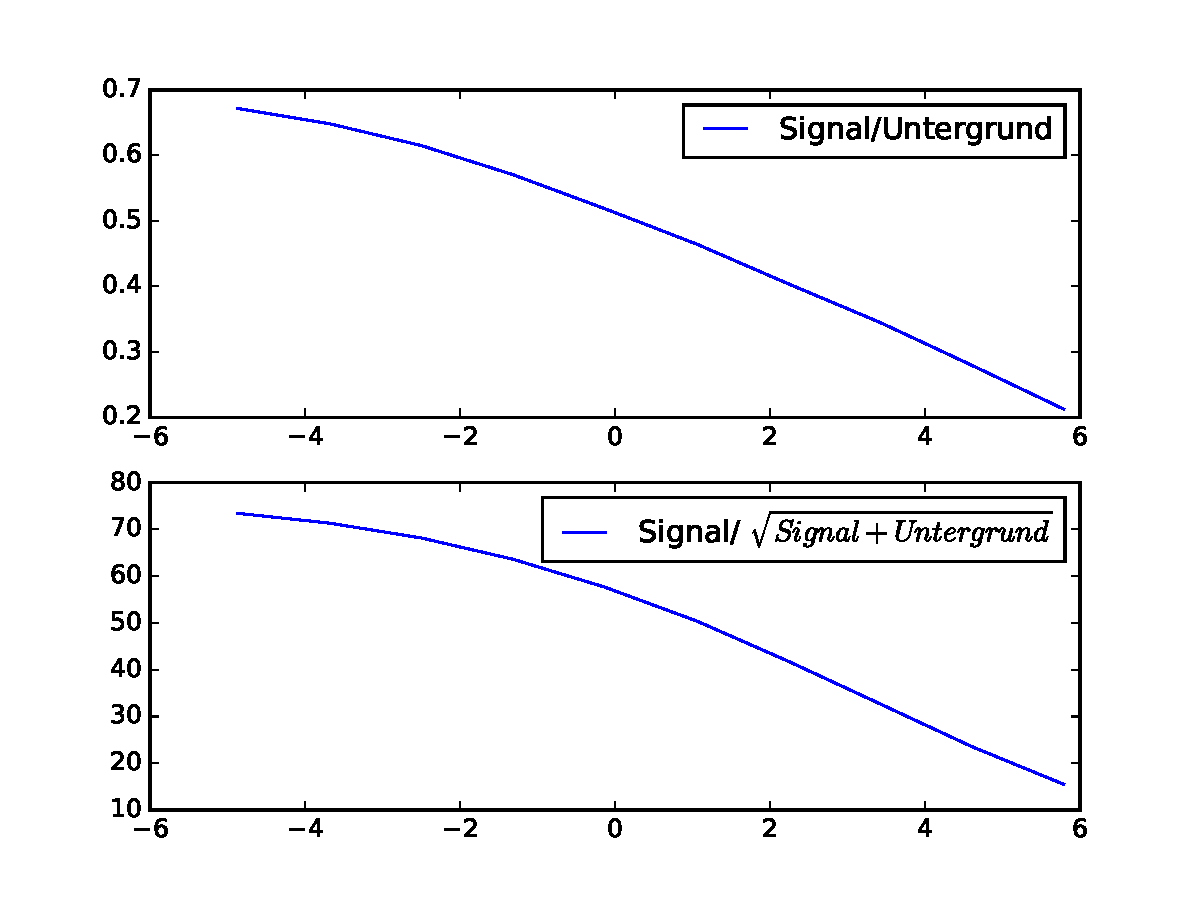
\includegraphics[height=7cm]{./Figures/SigZuUnt2.pdf}
  \caption{Signal zu Untergrundverhältnis sowie Signifikanz}
\end{figure}


%Aufgabe 2
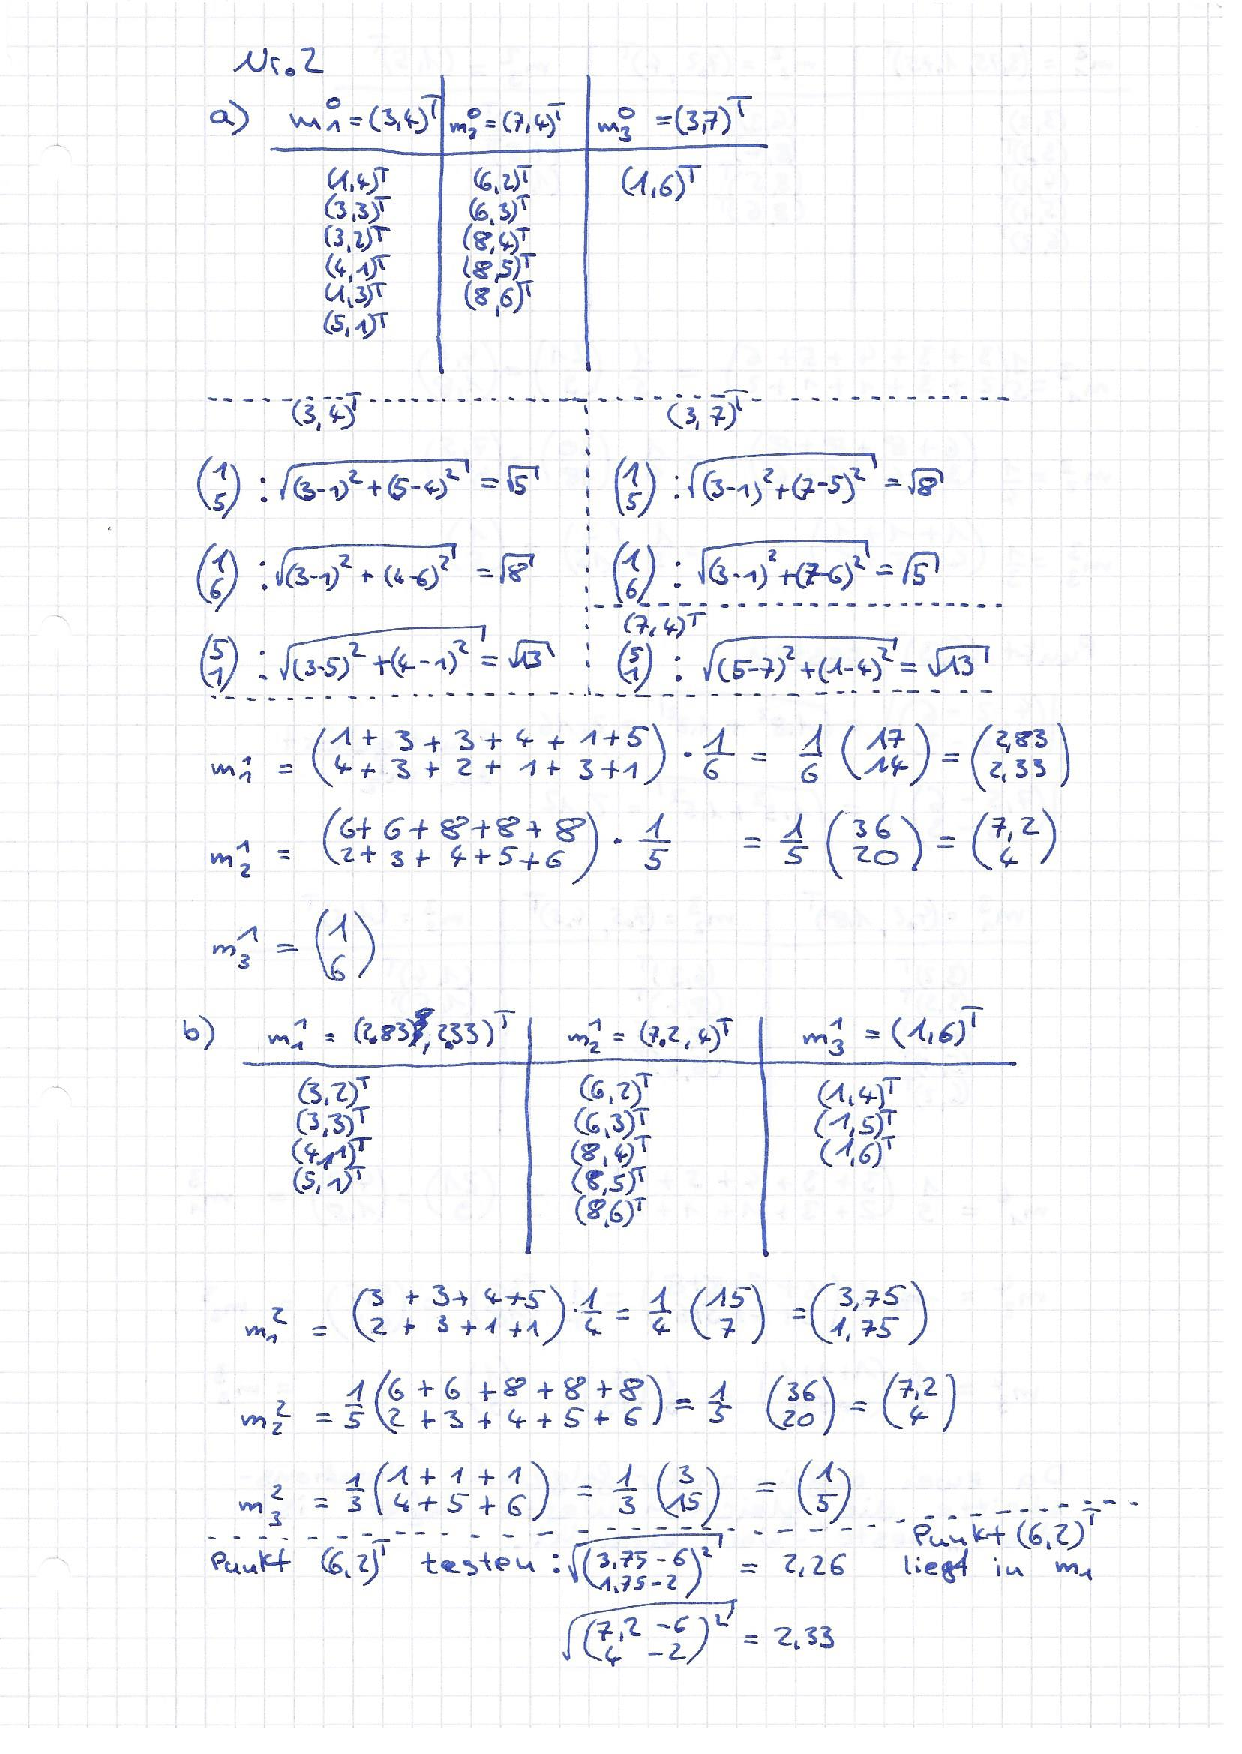
\includepdf[pages={1}]{Figures/Aufgabe_2a.pdf}
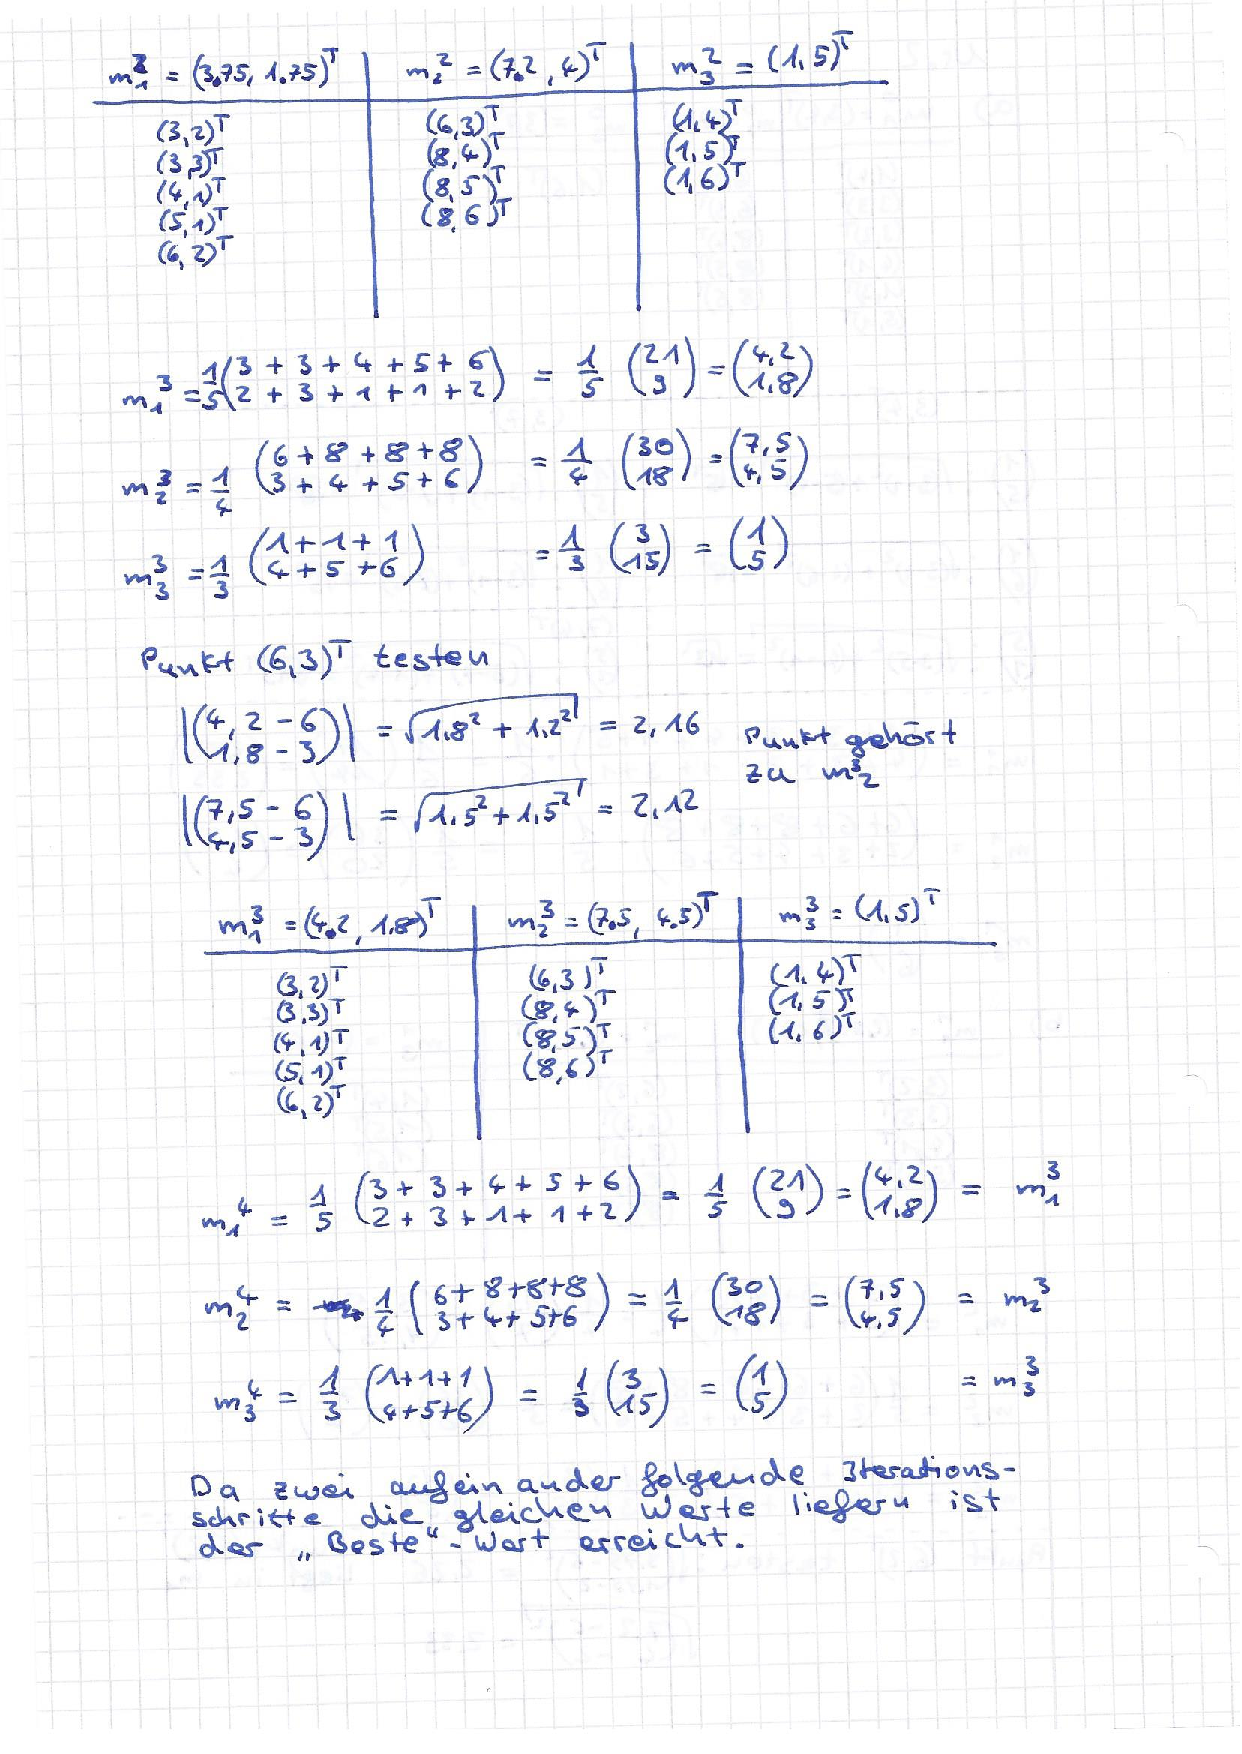
\includepdf[pages={1}]{Figures/Aufgabe_2b.pdf}
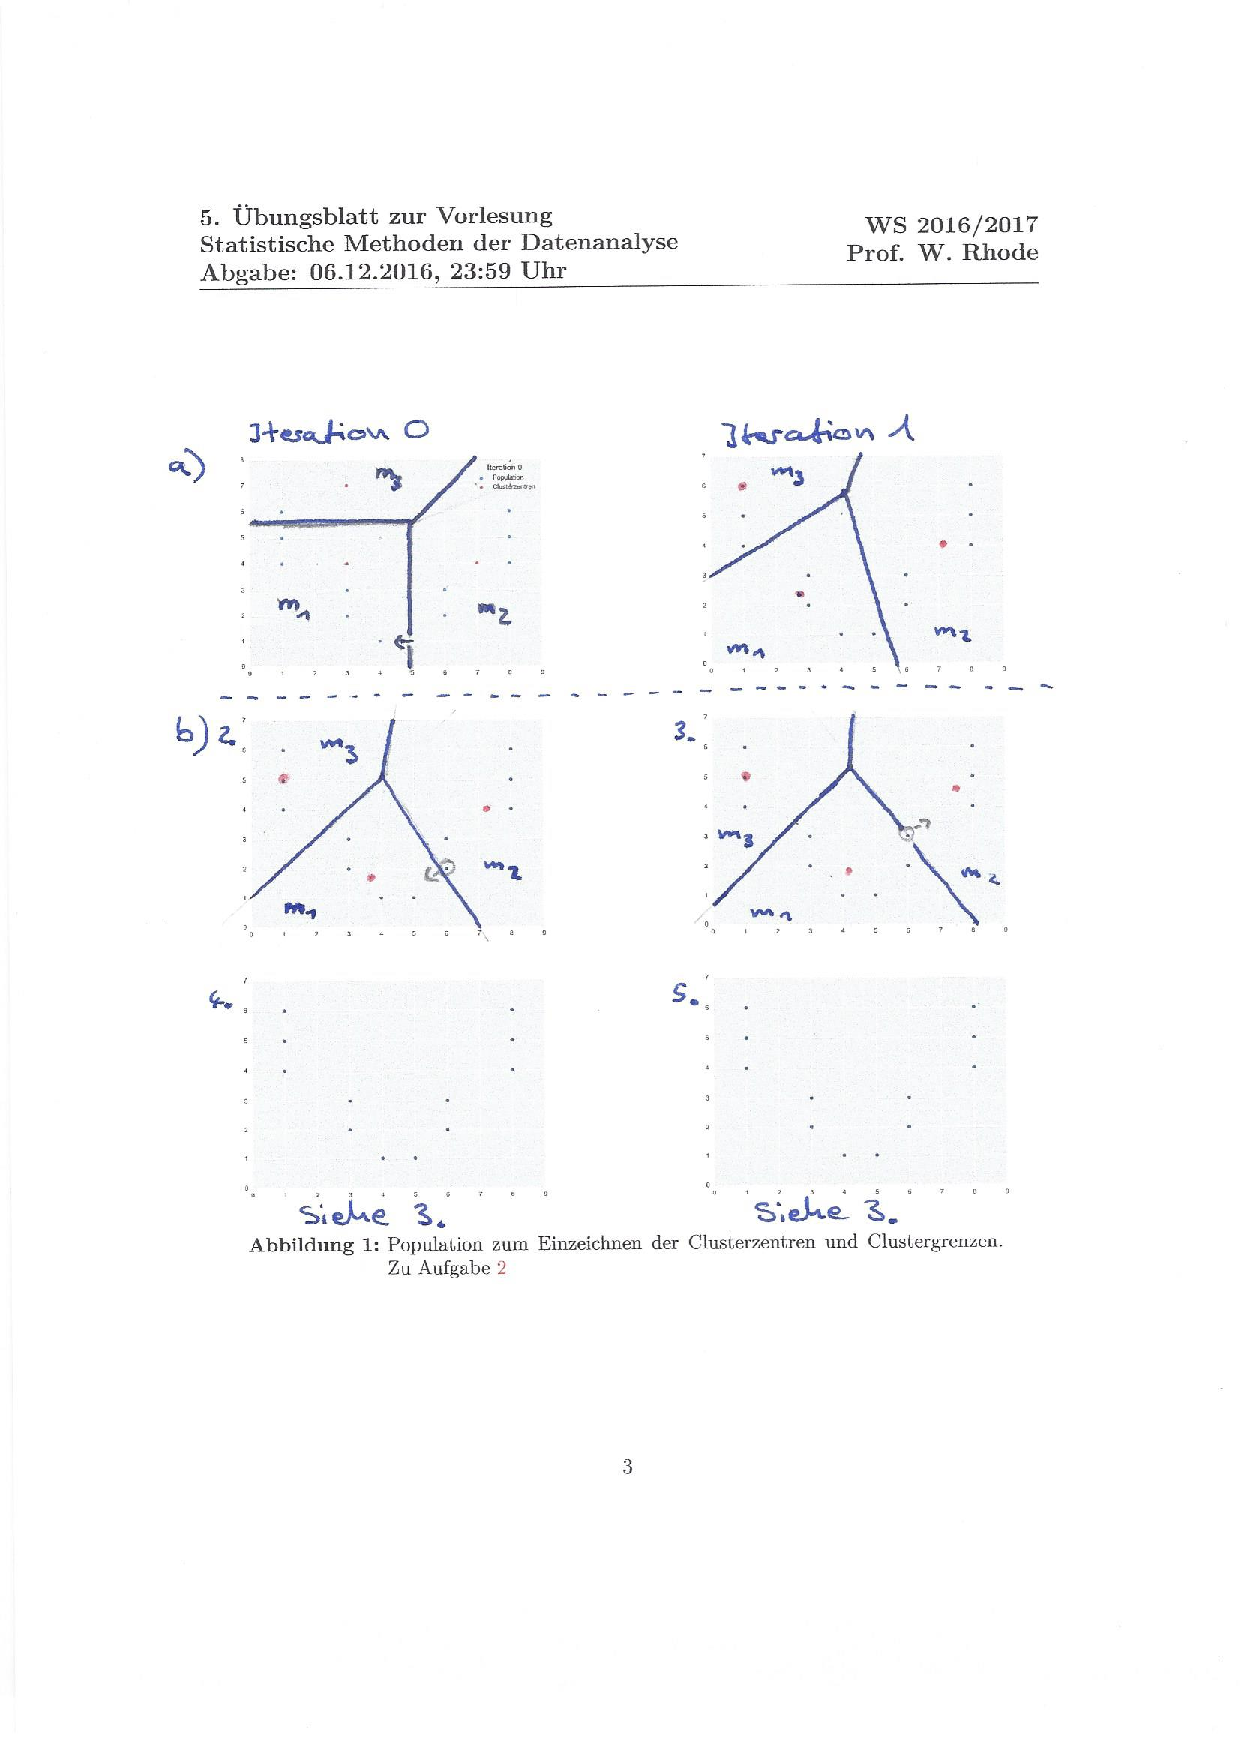
\includepdf[pages={1}]{Figures/Aufgabe_2.pdf}


\section*{Aufgabe 3}
\subsection*{Einlesen und aussortieren der Daten}
\begin{figure}[H]
  \centering
  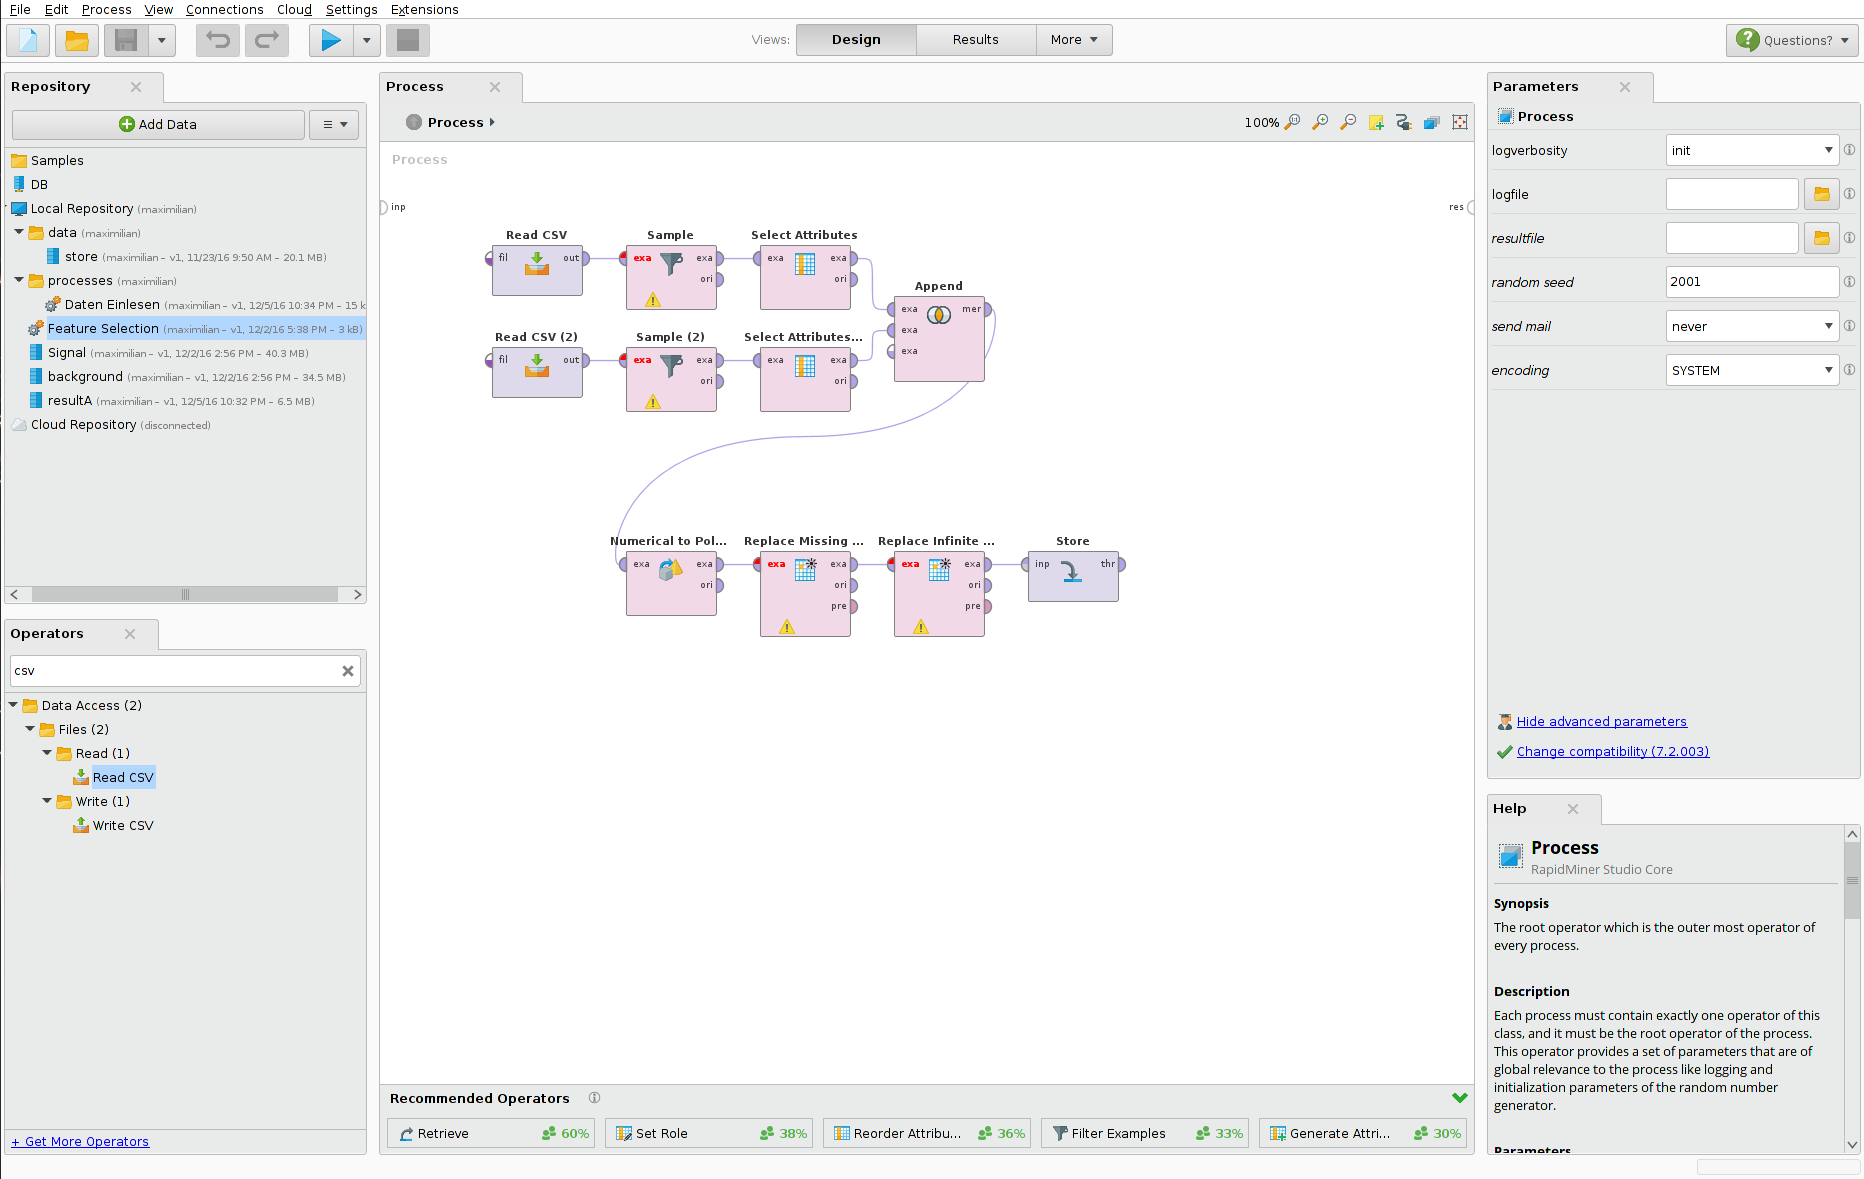
\includegraphics[height=10cm]{./Figures/Aufgabe3a.png}
\end{figure}
\subsection*{Feature Selection}
\begin{figure}[H]
  \centering
  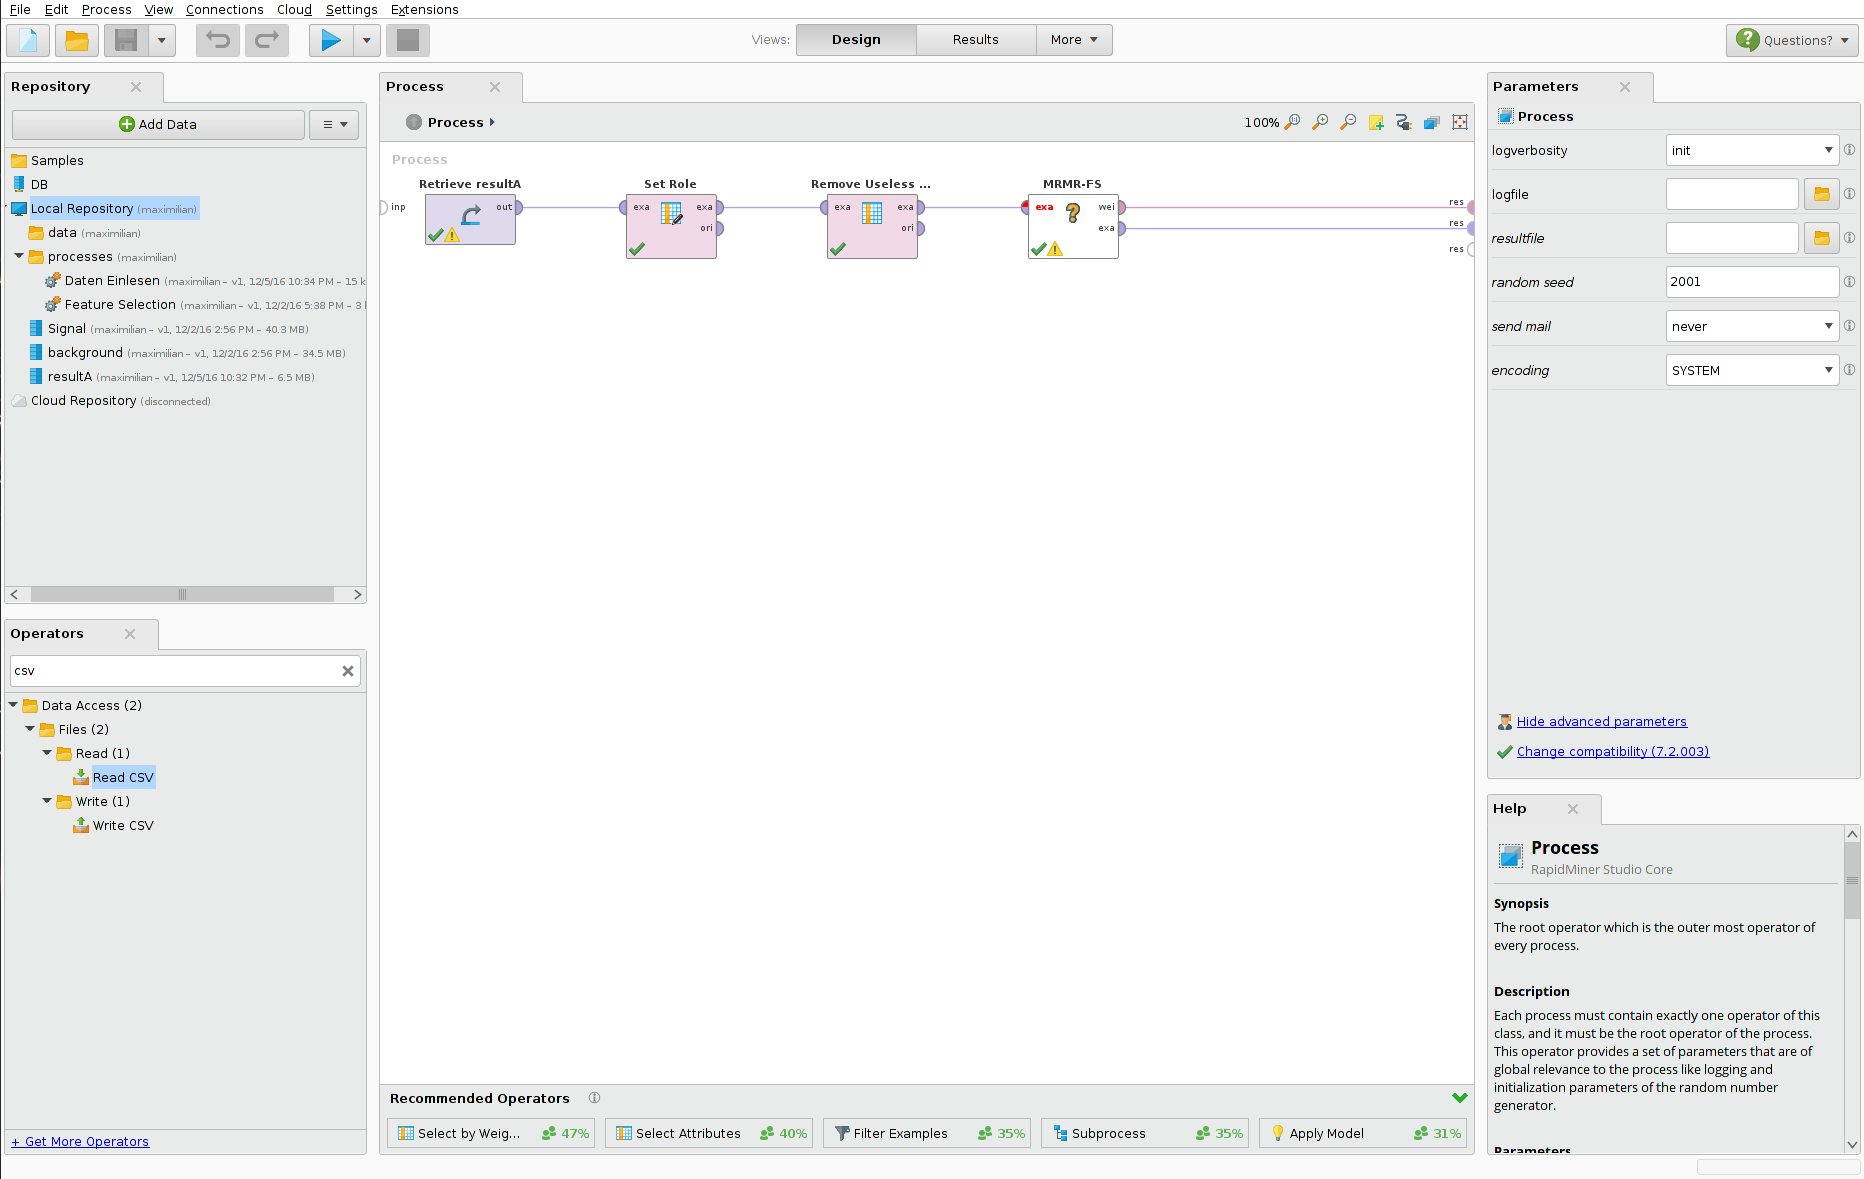
\includegraphics[height=10cm]{./Figures/Aufgabe3b.png}
\end{figure}
\subsection{Stabilität}
\begin{figure}[H]
  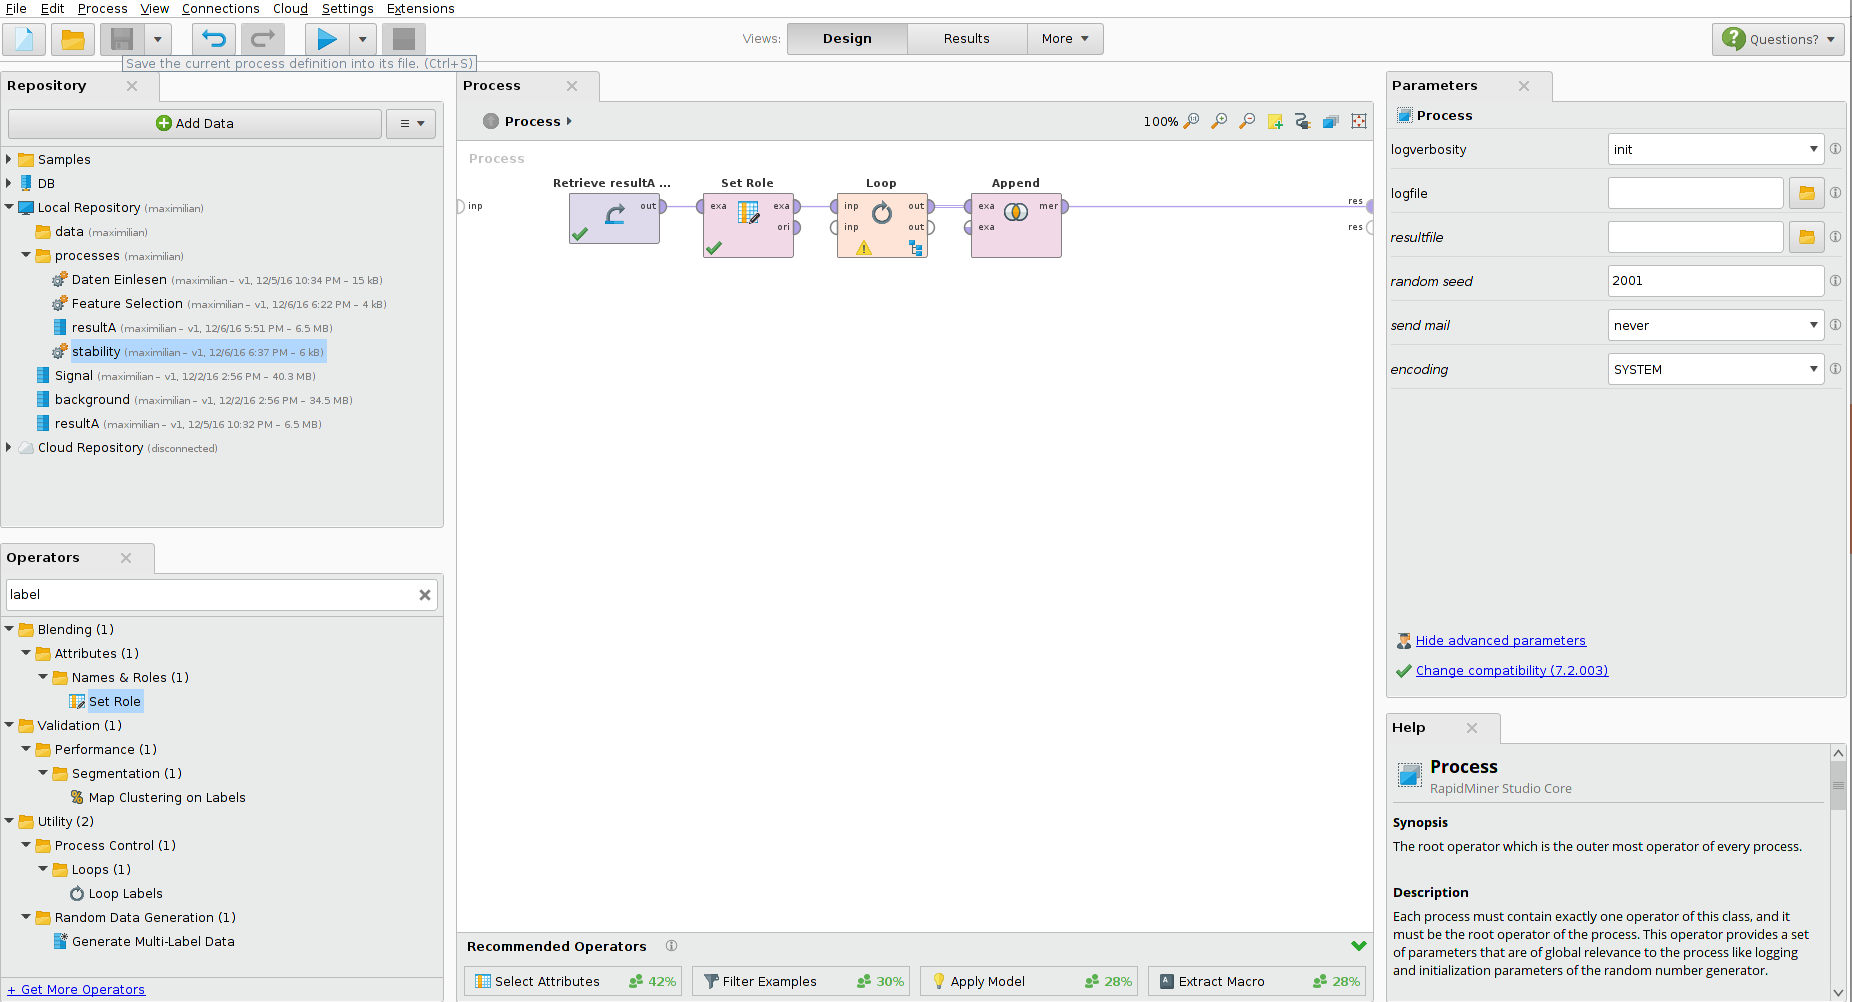
\includegraphics[height=7cm]{./Figures/Aufgabe3c1.png}
  \centering
\end{figure}
\begin{figure}[H]
  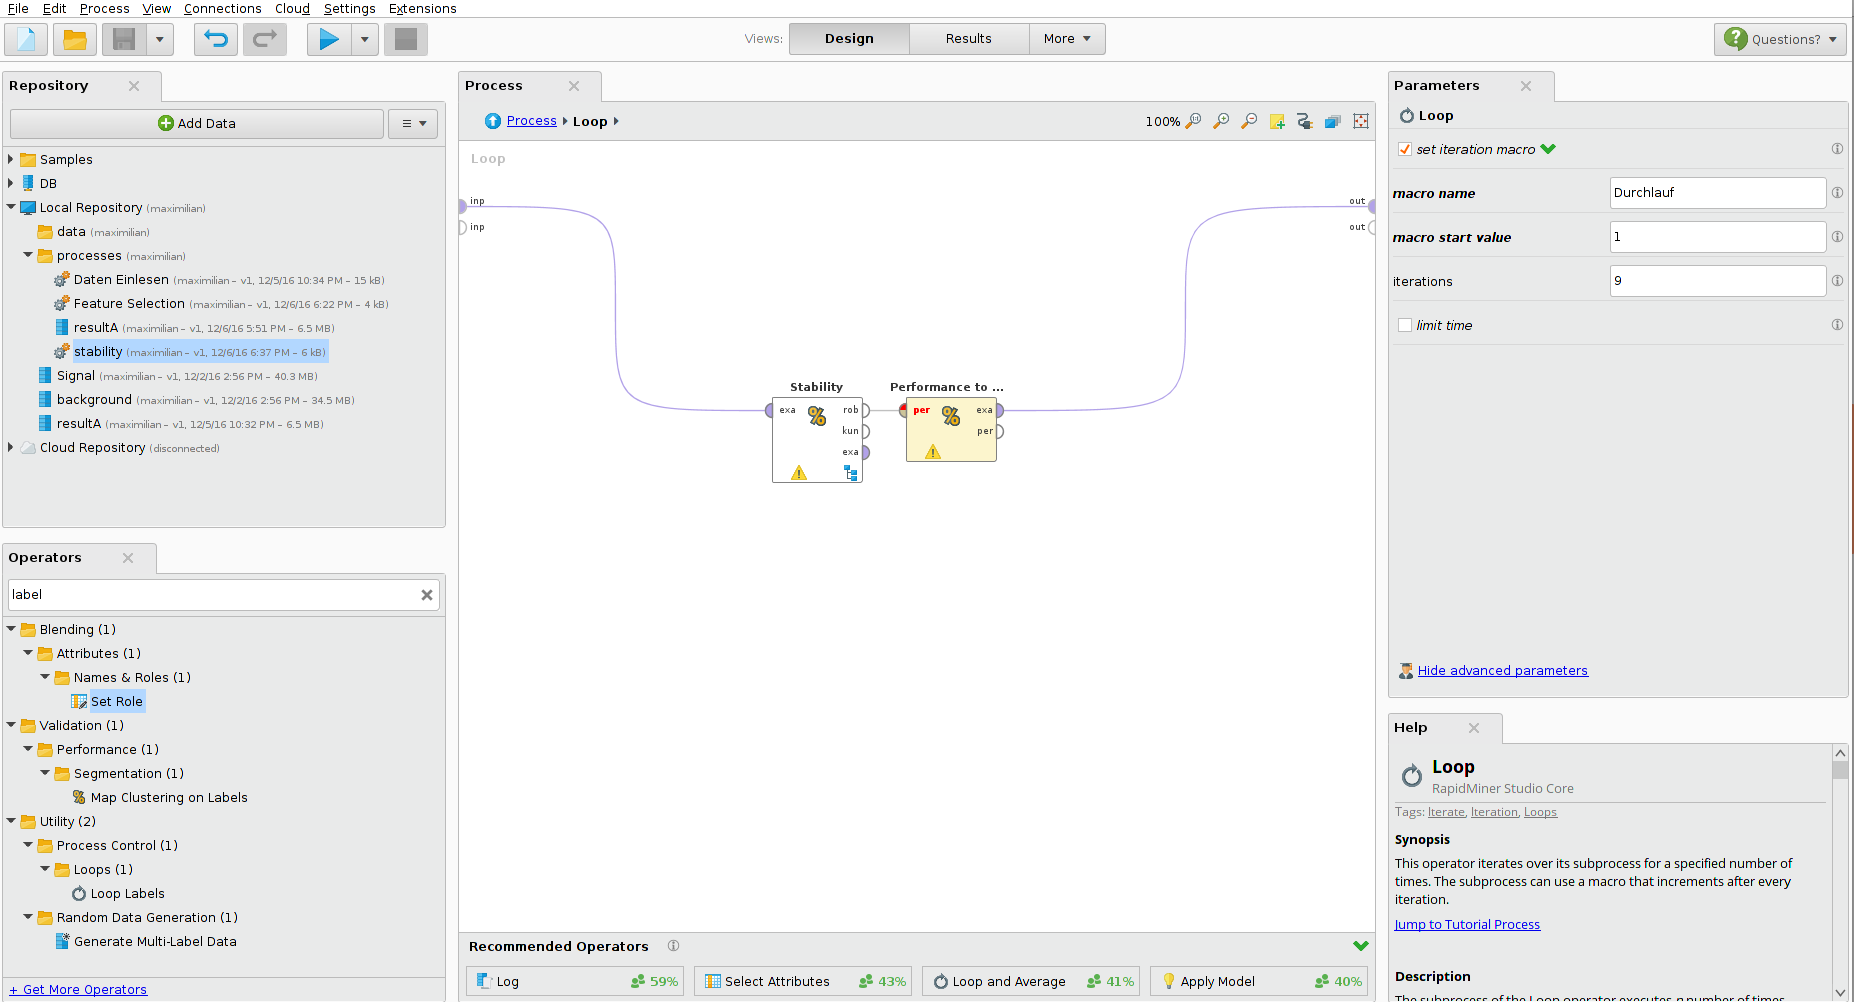
\includegraphics[height=7cm]{./Figures/Aufgabe3c2.png}
  \centering
\end{figure}
\begin{figure}[H]
  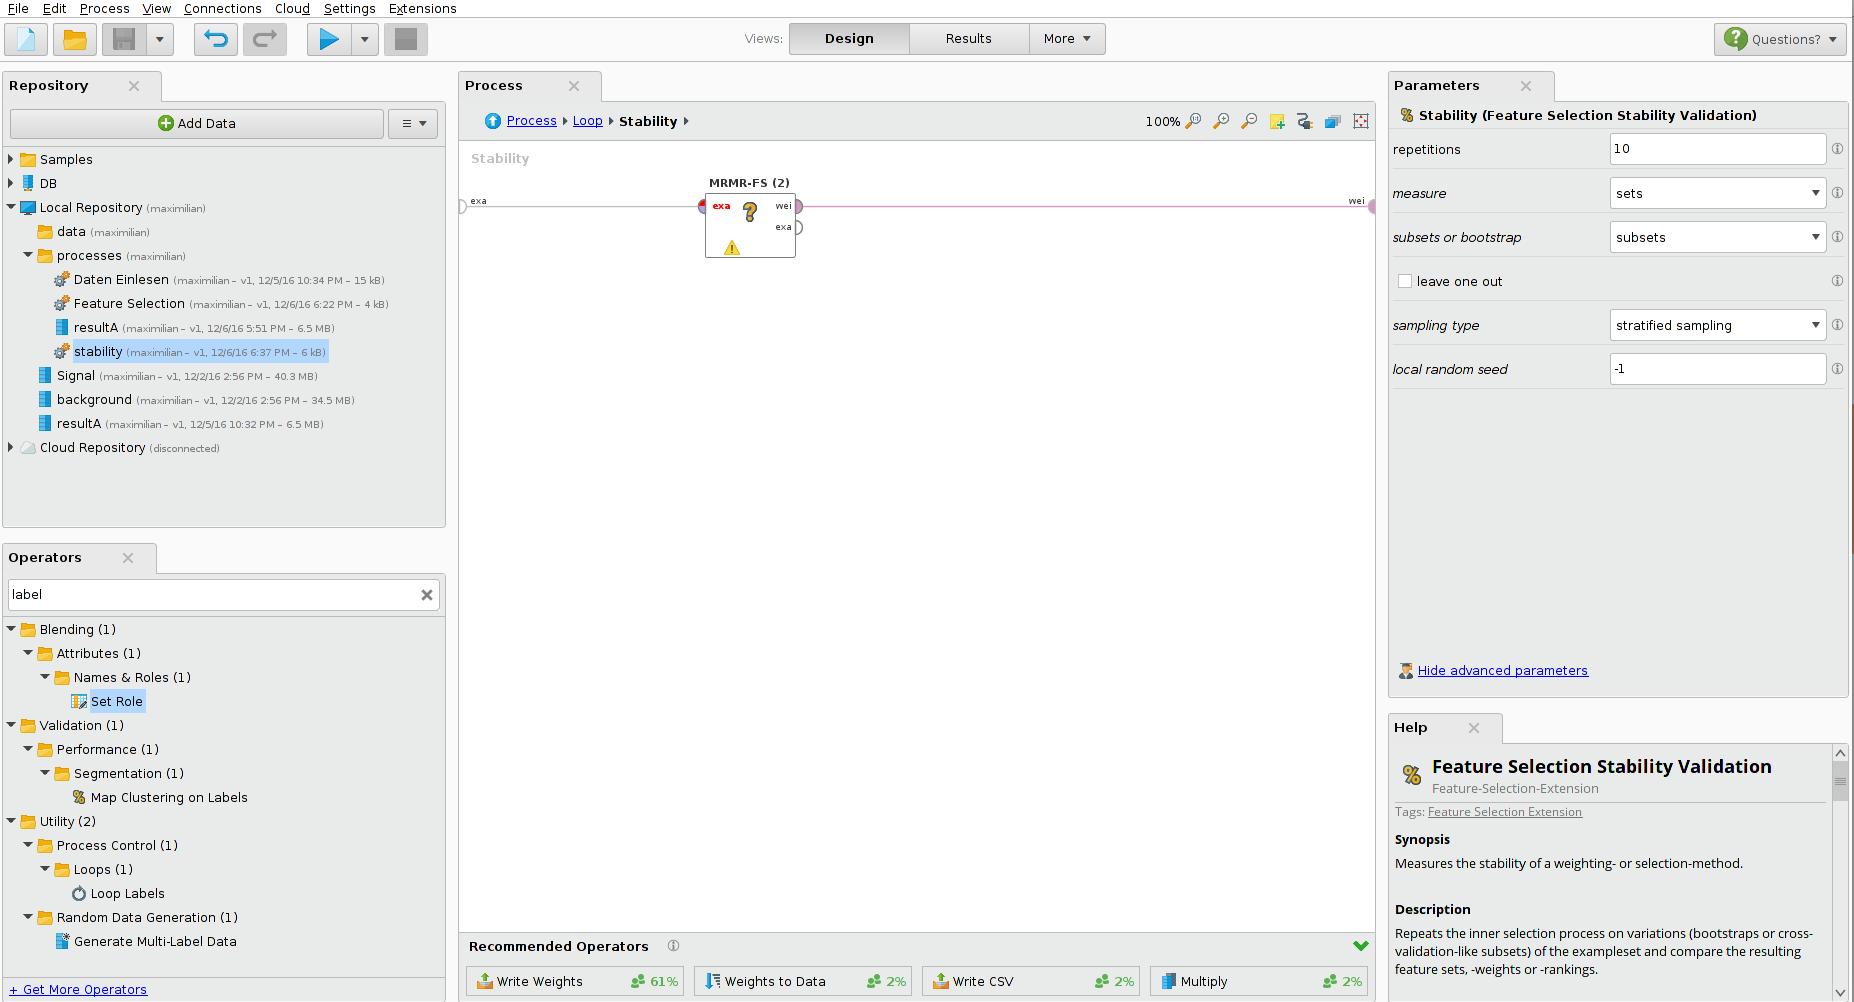
\includegraphics[height=7cm]{./Figures/Aufgabe3c3.png}
  \centering
\end{figure}
